\documentclass[mathserif,18pt,xcolor=table]{beamer}

\usepackage {bbm}
\usepackage {textpos}
\usepackage{tikz}
\usepackage{hyperref}
\usepackage{color}
\usepackage{amsmath}
\usepackage{amssymb}
\usepackage{soul}
\usepackage[compatibility=false]{caption}
\usepackage{subcaption}
\usepackage{multimedia}
\usepackage{multirow}



\definecolor{utorange}{RGB}{203,96,21}
\definecolor{utblack}{RGB}{99,102,106}
\definecolor{utbrown}{RGB}{110,98,89}
\definecolor{utsecbrown}{RGB}{217,200,158}
\definecolor{utsecgreen}{RGB}{208,222,187}
\definecolor{utsecblue}{RGB}{127,169,174}

\newcommand{\norm}[1]{\left\lVert #1 \right\rVert}

\mode<presentation>
{
  % \usetheme{Pittsburgh}   
  \usetheme{Boadilla}  
  \usefonttheme[onlymath]{serif}

  \setbeamercovered{invisible}
  \setbeamertemplate{navigation symbols}{}

  % Color Theme 
    \setbeamercolor{normal text}{bg=white,fg=utblack}
  \setbeamercolor{structure}{fg=utorange}

  \setbeamercolor{alerted text}{fg=red!85!black}

  \setbeamercolor{item projected}{use=item,fg=black,bg=item.fg!35}

  \setbeamercolor*{palette primary}{use=structure,fg=white, bg=utorange}
  \setbeamercolor*{palette secondary}{use=structure,bg=utsecbrown}
  \setbeamercolor*{palette tertiary}{use=structure,bg=utsecgreen}
  \setbeamercolor*{palette quaternary}{use=structure,fg=structure.fg,bg=utsecblue}

  % \setbeamercolor*{frametitle}{use=structure,fg=utorange, bg=utsecbrown}
  \setbeamercolor*{framesubtitle}{fg=utbrown}

  \setbeamercolor*{block title}{parent=structure,fg=black,bg=utsecgreen}
  \setbeamercolor*{block body}{fg=black,bg=utblack!10}
  \setbeamercolor*{block title alerted}{parent=alerted text,bg=black!15}
  \setbeamercolor*{block title example}{parent=example text,bg=black!15}

  \setbeamerfont{framesubtitle}{size=\small}
}

\usepackage[orientation=landscape,size=custom,width=16,height=9.75,scale=0.5,debug]{beamerposter}
% \usepackage[orientation=landscape,size=custom,width=16,height=9,scale=0.5,debug]{beamerposter}


\makeatletter
\setbeamertemplate{footline}
{
  \leavevmode%
    \hbox{%
      \begin{beamercolorbox}[wd=.333333\paperwidth,ht=2.25ex,dp=1ex,center]{author in head/foot}%
        \usebeamerfont{author in head/foot}\insertshortauthor%~~\beamer@ifempty{\insertshortinstitute}{}{(\insertshortinstitute)}
      \end{beamercolorbox}%
        \begin{beamercolorbox}[wd=.5\paperwidth,ht=2.25ex,dp=1ex,center]{title in head/foot}%
        \usebeamerfont{title in head/foot}\insertshorttitle
        \end{beamercolorbox}%
        \begin{beamercolorbox}[wd=.166666\paperwidth,ht=2.25ex,dp=1ex,right]{date in head/foot}%
        \usebeamerfont{date in head/foot}\insertshortdate{}\hspace*{2em}
        \insertframenumber{} / \inserttotalframenumber\hspace*{2ex} 
      \end{beamercolorbox}}%
        \vskip0pt%
}
\makeatother

\usepackage{kerkis}
\usepackage[T1]{fontenc}
\usepackage[protrusion=true,expansion=true]{microtype}
\usepackage{amsmath}


\renewcommand*{\thefootnote}{\fnsymbol{footnote}}


\pgfdeclareimage[height=1.0cm]{utbig}{logos/UTWordmark.pdf}
\pgfdeclareimage[height=0.6cm]{ut}{logos/UTWordmark.pdf}

\title{Stacked Denoising Autoencoders}
\subtitle{SGD and GA}
\author[Jason Liang and Keith Kelly]{ {Jason~Liang, Keith~Kelly} \\  
}

\institute{UT-Austin\\ \mbox{}  \\  \pgfuseimage{utbig} }
\date[ACHA]

\begin{document}

\tikzstyle{block} = [rectangle, draw, rounded corners, shade, top color=white, text width=5em,
  bottom color=blue!50!black!20, draw=blue!40!black!60, very thick, text centered, minimum height=4em]
  \tikzstyle{line} = [draw, -latex']
  \tikzstyle{cloud} = [draw, ellipse,top color=white, bottom color=red!20, node distance=2cm, minimum height=2em]


  \beamertemplateballitem
  %\beamertemplatetransparentcoveredhigh

  \frame{\titlepage}

  \addtobeamertemplate{frametitle}{}{%
      \begin{textblock*}{100mm}(0.95\textwidth,-0.75cm)
    \pgfuseimage{ut}
    \end{textblock*}
  }


% ------------------------------------------------------------
\begin{frame}[t]
\frametitle{Intro}
\framesubtitle{~~}  %% needed for proper positioning of the logo ...

Slides online at

\href{http://users.ices.utexas.edu/~keith/files/MLProject.html}{\textcolor{blue}{http://users.ices.utexas.edu/\textasciitilde keith/files/MLProject.html}}


\end{frame}

%%%%%%%%%%%%%%%%%%%%%%%%%%%%%%%%%%%%%%
%% Frame
%%%%%%%%%%%%%%%%%%%%%%%%%%%%%%%%%%%%%%

\begin{frame}[t]
	\frametitle{Introduction}
	\framesubtitle{~~}  %% needed for proper positioning of the logo ...

\begin{figure}[h]
	\centering
	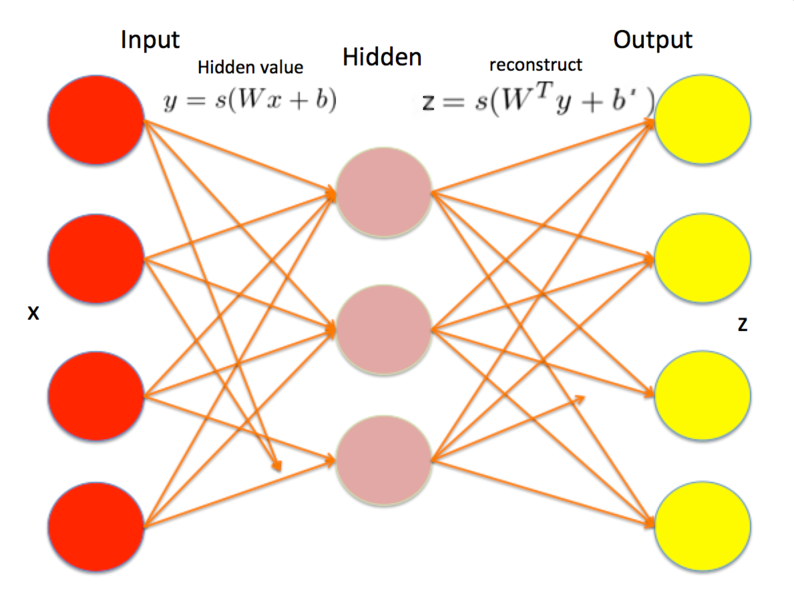
\includegraphics[width=0.7\linewidth]{autoencoder.png}
	\caption{Overview of an autoencoder and its encoding, decoding stages. The weight matrix of the decoding stage is the transpose of the weight matrix of the encoding stage.}
	\label{fig:autoencoder}
\end{figure}


\end{frame}
%%%%%%%%%%%%%%%%%%%%%%%%%%%%%%%%%%%%%
%% Frame
%%%%%%%%%%%%%%%%%%%%%%%%%%%%%%%%%%%%%%
\begin{frame}[t]
	\frametitle{Introduction}
	\framesubtitle{~~}  %% needed for proper positioning of the logo ...

\end{frame}





%%%%%%%%%%%%%%%%%%%%%%%%%%%%%%%%%%%%%%
%% Frame
%%%%%%%%%%%%%%%%%%%%%%%%%%%%%%%%%%%%%%
\begin{frame}[t]
	\frametitle{Conclusions}
	\framesubtitle{~~}  %% needed for proper positioning of the logo ...


\end{frame}



%%%%%%%%%%%%%%%%%%%%%%%%%%%%%%%%%%%%%%
%% Frame
%%%%%%%%%%%%%%%%%%%%%%%%%%%%%%%%%%%%%%
\begin{frame}[t]
	\frametitle{Future work}
	\framesubtitle{~~}  %% needed for proper positioning of the logo ...


\end{frame}




\end{document}


